%%%%%%%%%%%%%%%%%%%%%%%%%%%%%%%%%%%%%%%%%%%%%%%%%%%%%%%%%%%%%%%%%%%%%%%%%%%%%%%%

\documentclass[letterpaper, 10 pt, conference]{ieeeconf}  
                                                          
%\documentclass[a4paper, 10pt, conference]{ieeeconf}      
                                                          
\overrideIEEEmargins

% The following packages can be found on http:\\www.ctan.org
%\usepackage{graphics} % for pdf, bitmapped graphics files
%\usepackage{epsfig} % for postscript graphics files
\usepackage{mathptmx} % assumes new font selection scheme installed
%\usepackage{times} % assumes new font selection scheme installed
\usepackage{amsmath} % assumes amsmath package installed
\usepackage{amssymb}  % assumes amsmath package installed
\usepackage{float}
\usepackage{array}
\usepackage[spanish]{babel}
\usepackage{comment}
\usepackage{graphicx}


\title{\LARGE \bf
Symbol Digital Modalities Test (SDMT) a Mobile App Study Analysis
}

\author{Pim van Oirschot, Pedro Vladimir Hern\'andez Serrano}
\begin{document}

\maketitle
\thispagestyle{empty}
\pagestyle{empty}


%%%%%%%%%%%%%%%%%%%%%%%%%%%%%%%%%%%%%%%%%%%%%%%%%%%%%%%%%%%%%%%%%%%%%%%%%%%%%%%%
\begin{abstract}

On this document we will find the description of the Symbol Digital Modalities Test (SDMT), and how is been used for detect impairment on Multiple Sclerosis (MS) patients. It is going to be showed the experiment conducted with 23 volunteers, 15 HC and 8 MS, which they scored 
It was replicated the stages of reliability and validity

\end{abstract}

%%%%%%%%%%%%%%%%%%%%%%%%%%%%%%%%%%%%%%%%%%%%%%%%%%%%%%%%%%%%%%%%%%%%%%%%%%%%%%%%
\section{Introduction}
\vspace{2mm}

Cognitive impairment is one of the traits observed in 43-65\% of Multiple Sclerosis (MS) patients. Many batteries have been proposed to diagnose the cognitive impairment in MS. The alternative showed in this document is the use of Symbol Digital Modalities Test (SDMT), which only takes 90 seconds and aims to measure the information processing speed. As the name of the SDMT suggests, the subject is presented with a map of symbols and digits and asked to match symbol and digits. The total number of the correctly classified digits, reaction time and the total number of digits are noted for analysis.

The SDMT has proven to be quite useful in neuropsychological MS research. It has excellent test-retest reliability, and alternate forms have been developed that are equivalent in difficulty. When the alternate forms are used, reliability is maintained. Validity research shows that SDMT is a good measure of processing speed or efficiency. The test very effectively represents the domain of processing speed.

The main difference of responding the SDMT test on paper and responding on digital is that the second one we have the precise moment every patient performs a task, so we might discover new features as time. We are interested in analysing the time of response every participant have, in addition, we want to check the practicing effect on trials over the time.

%%%%%%%%%%%%%%%%%%%%%%%%%%%%%%%%%%%%%%%%%%%%%%%%%%%%%%%%%%%%%%%%%%%%%%%%%%%%%%%%
\section{Methods}
\vspace{2mm}

\subsection{Study}
\vspace{2mm}

It's been conducted a study with 23 volunteers with different demographics, distributed on 15 Healthy individuals (65.0\%)and 8 individuals with a type of MS (35.0\%) . The Study performed from 2017-05-31 to 2017-08-10 and it's been instructed the people to respond the test through the application with restriction of time of the day.

We expect that every person performs the test within 8 or 10 times, we found that the participants actually respond 9.47 times on average alongside the study. The number of days of the study on every participant should be 30 days, we found out 31.55 the length of actual time the test was performed on every participant $(9.47∗3.33=31.55)$ The expected number of trials times the expected days between every trial we can find an inference for the days.

It's been chosen the score variable as the number of correct answers on every test, but also we recorded metrics regarding on time of response to every task in the test. We found that the average time of response on the MS group was 3.82 Seconds and 3.35 Seconds for the Healthy group.

In the study we also found the difficulty of the symbols in the test, sorted by the average time of response on each different symbol, and the order from thee most difficult (more time to response, 2.1 Seconds ), to the easiest one (the less time to response 1.6 Seconds), as follows: 1. Mult, 2. Star, 3. Plus, 4. Triangle, 5. Inf, 6. Square, 7. Hamburger, 8. Window, 9. Circle. Is important to say that this sequence is the same with MS individuals and HC group.

\subsection{Statistics}
\vspace{2mm}

The individuals in the study responded the test different number of times, we call every time a person make the test is an event, and if we summarize the number of event between the two groups we have for MS Group 11.93 (SD 4.59) of times that an individual make the test and 8.38 (SD 3.11) times for HC Group.

Regarding with the score variable itself, we got Average Score of MS Group: 46.22 (SD 7.88) with a Standard Error of (SEM 2.03), therefore computing intervals it's been obtained a True Score Interval as follows [42.23, 50.21]. The same calculations were performed on the Health individuals, we found an Average Score of 52.92 (SD 8.22)
with a Standard Error of (SEM 2.91) making the True Score Interval over [47.22, 58.613].

Using the same logic we can plot the distributions of both groups, considering all the events of the participants, then  we might perform a test to prove that all the scores of MS patients have a normal distribution, the same with HC participants, at this point it does not seems to be any difference in standard deviation on both groups.

\begin{figure}[ht]
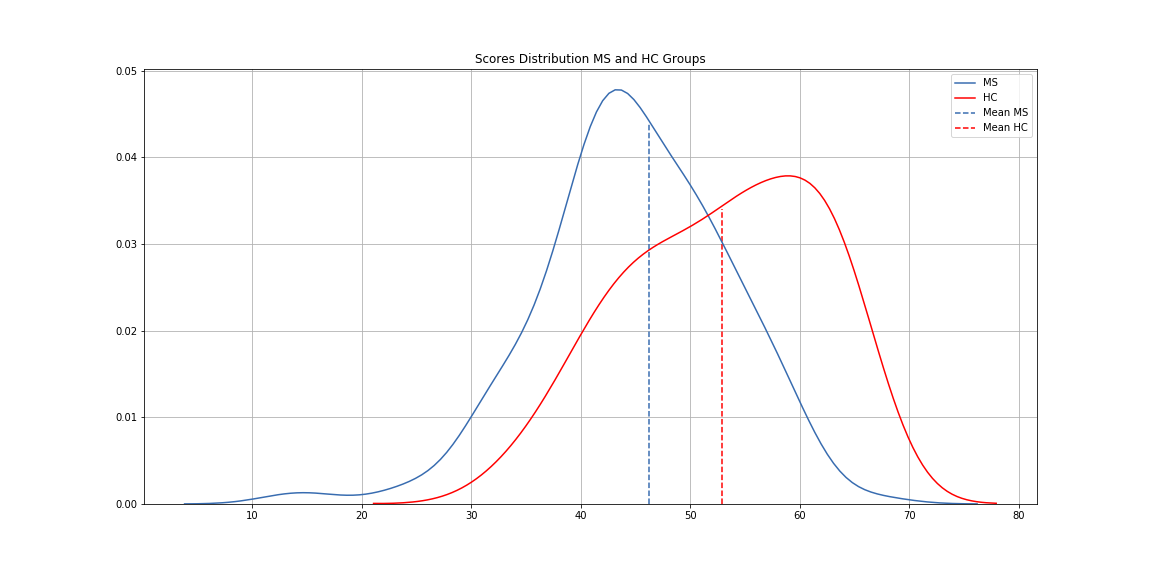
\includegraphics[width=9cm]{scores_distribution_grid.png}
\caption{Scores Distribution}
\label{tab:scores}
\end{figure}

\vspace{2mm}
\input{table1}

%%%%%%%%%%%%%%%%%%%%%%%%%%%%%%%%%%%%%%%%%%%%%%%%%%%%%%%%%%%%%%%%%%%%%%%%%%%%%%%%
\section{Results}
\vspace{2mm}

\subsection{Test-Restest Reliability}
\vspace{2mm}

Benedict et al. BMC Neurology 2012 recomends a Test-Retest Reliability Assessment to be achieved by evaluatingan MS and/or healthy volunteer sample on two occasions separated by 1–3 weeks. This is thegold standard separation where the question is only test reliability, then Pearson’s correlation coefficient > 0.70 will usually be required. On this study was found an Average Days Between Test-retest: 14.7 (SD): 3.21, therefore it fits with the recomendation. We found the scores on SDMT Test-Retest Reliability as follows:

Average score MS Group $0.84$ $p=0.0000849$ 

Average score HC Group $0.85$ $p=0.00693$ 

The Standard Error of Measurement (SEM) was calculated for every group, therefore we obtain $SEM_{MS}=2.274$ and $SEM_{HC}=2.004$

\begin{figure}[ht]
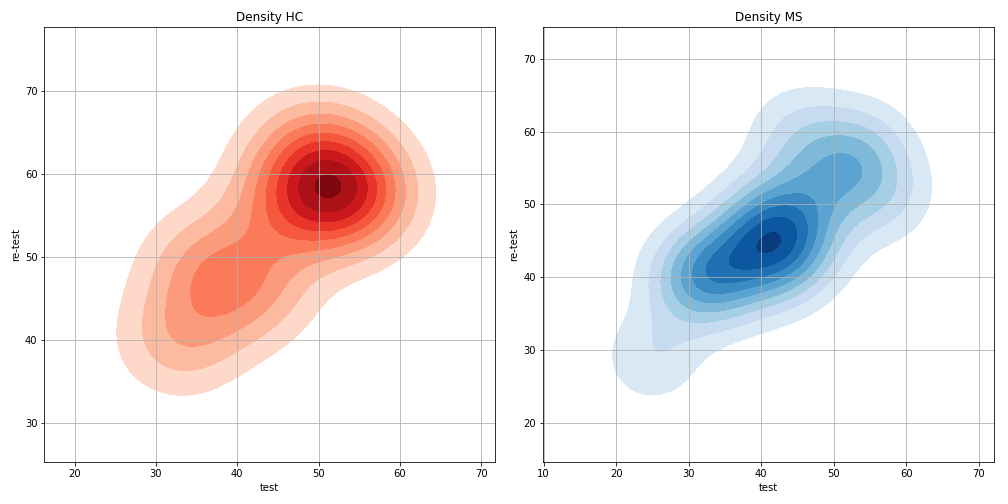
\includegraphics[width=8cm]{test-retest_density_grid.png}
\caption{Test Re-test Density}
\label{tab:density}
\end{figure}

It is possible to see the correlation between test and retest on both groups, also is intuitive to see that people are scoring more on the second one, showing an effect of improving with the time. In the other hand we calculate the Minimal Detectable Change (MDC), that is representing the magnitude of change necessary to exceed the measurement the error of two repeated measures at a specified CI was calculated for the 95\% CI as:
$$MDC_{95} = SEM( 1.96 )(\sqrt{2})$$. It's been found for each group $MDC_{MS}= 6.304$ and $MDC_{HC}=5.556$ which means that if a measure is more than that it's a possible outlier.

\subsection{Effect Size}
\vspace{2mm}

The first difference in means we looked for is between the two groups, MS and HC, using the $Cohen`s d-value$, compared with the results of Benedict 2016, obtained $d=1.11$ which is considered a Large difference in means (Cohen, 1988), we found  $d=0.837$ which is considered Large too. After that we calculate the scores on different moment of the day, in order to see if there's a difference in performance.

\input{table2}

There's not significance difference between means, so it means that a person is going to score alike no matter the moment on the day. But in the other hand is clearly to see that respond in the morning for MS group is presumably less variant

Difference in Variance for MS: $66.52\%$  $p=0.0285$

Difference in Variance for HC: $97.0\%$  $p=0.466$

There is an statistical significant difference between the variance between morning and afternoon on MS group, it means that people perform more constant over the time if they respond in the morning, in the other hand, it shows also a big difference for HC, but we got a big p-value, so we cannot reject the null hypothesis for HC group

\subsection{Practicing Effect}
\vspace{2mm}

The Effect on Median Time of Response it is been split on MS and HC groups trying to find a statistical difference on the first median time a person performed and the last median time the person performed, we used the d-Cohen value to find an effect. 

Cohens d-value, First Median vs Last Median: 
 MS: 0.754 Large 
 HC: 0.974 Large

Average Score of MS Group: 
 First: 4186.53 (SD 803.87) 
 Last: 4186.53 (SD 803.87) 
Cohens d-value: 0.415   Ttest pvalue=0.0802

Average Score of HC Group: 
 First: 3798.62 (SD 631.04) 
 Last: 3798.62 (SD 631.04) 
Cohens d-value: 1.037   Ttest pvalue=0.000176

In order to prove validity, we need to be able to predict who is an MS person called Predictive validity, it means the degree to which a test accurately predicts a criterion that will occur in the future. 

Source	Accuracy	Specificity	Sensitivity
Akbar 2011	0.78	0.84	0.71
Ruet 2013	0.77	0.85	0.60
Van Schependom 2014	NA	0.60	0.91
Orikami
Inference	0.67	0.69	0.66
k-NN	0.79	0.80	0.79
Naive Bayes	0.79	0.80	0.79
Logistic	0.84	0.85	0.84

\begin{figure}[ht]
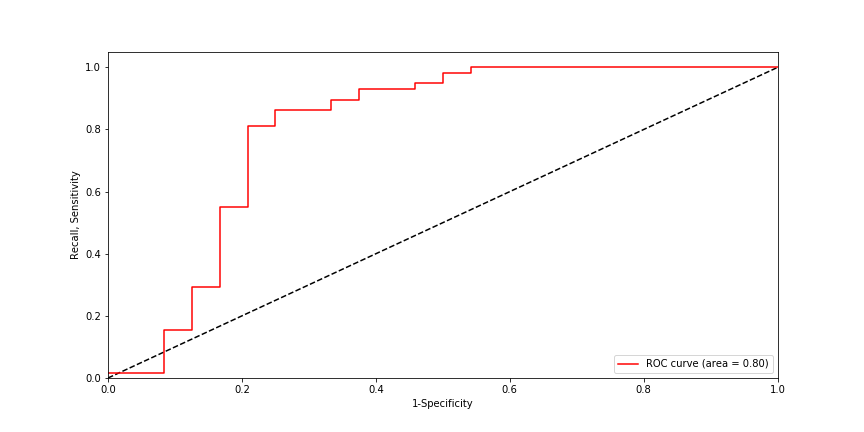
\includegraphics[width=9cm]{roc_logistic.png}
\caption{ROC Logistic}
\label{tab:roc}
\end{figure}


\section{Discussion}

On the study the recomendations it's been followed in order to accomplish the correct Reliability of the expermiment and after watch the results we might say that the test is Reliable there's only the consideration on the number of participants to perform the study

In the literature there's more than one method to measure the difference between the statistic of two populations, on this study it is been used the d-Cohen's value and the F test for difference in variance

We reject the null hypothesis on MS group, so it means that there is 68\% greater the variance of scores if the patients respond in the morning, rather than the afternoon.
In the other hand we can not reject the null hypothesis on the HC group because there's no much data points, that means that we might not say anything about how late the participant in HC perform the test

In the literature shows that exist practicing effect and more significant after longer testing period
Not influenced by gender, age, relapses, disability progression and prior natalizumab treatment
They conclude that the practicing effect is less if they are more impaired on the EDSS scale
\vspace{3mm}

Distraction Points as a MS Feature

It is mainly important to analyze all the features involved in every test taken by a person, and it is straightforward thinking that not all tasks are with full concentration because the nature of the tool, is an app, and we might expect the people taking the test can get distracted by some random reason
The main objective here is to analyze any pattern related to the time in milliseconds a participant spend on responding every visual task.

Standart Deviation of every delta per group 
 MS: 663.6751885085198 
 HC: 502.5068924690813
 
  One person, one event¶
We can just take one single event on a random choise person (eobt3CosDzEtxWW5P) for instance, and plot the time of response in milisecond alongside the 90 seconds showing the symbols choosen on each task

As we might see the points outside of the boundaries are distraction points because they are 2 SD of the median time of response, where the SD corresponds the variance of the group.

Group	Average Score	Average Distractions
MS	52.91	1.81
HC	46.22	1.49

As we may see on the plots above we see a negative and significative correlation, the MS group is more clear. The more distractions the less score
The number of distractions that a single person has is a clear feature that helps to classify the MS people, this feature does not deoend in demographic variables but just with in the test behaviour
\begin{figure}[ht]
\includegraphics[width=9cm]{distraction_sample.png}
\caption{Distraction Points}
\label{tab:dis}
\end{figure}

he general performance is acceptable, and at some point better than the references, tryying more type of validity is going to make clear the complete validity of the test
The next steps should be try concurrent validity correlating scores on MS people with impairment data, job information or fMRI results





%%%%%%%%%%%%%%%%%%%%%%%%%%%%%%%%%%%%%%%%%%%%%%%%%%%%%%%%%%%%%%%%%%%%%%%%%%%%%%%%


%%%%%%%%%%%%%%%%%%%%%%%%%%%%%%%%%%%%%%%%%%%%%%%%%%%%%%%%%%%%%%%%%%%%%%%%%%%%%%%%




\begin{thebibliography}{10}

\bibitem{c1} M. L\'opez-G/'ngora, L. Querol, and A. Escart/'in. A one-year follow-up study of the symbol digit modalities test (sdmt) and the paced auditory serial addition test (pasat) in relapsing-remitting multiple sclerosis: an appraisal of comparative longitudinal sensi- tivity. BMC Neurology, 15(1):1–8, 2015
\bibitem{c2} N. Akbar, K. Honarmand, N. Kou, and A. Feinstein. Validity of a computerized version of the symbol digit modalities test in multiple sclerosis. Journal of Neurology, 258(3):373–379, 2011.
\bibitem{c3} S. Hoffmann, M. Tittgemeyer, and D. Y. von Cramon. Cognitive impairment in multiple sclerosis. Current Opinion in Neurology, 20(3), 2007.
\bibitem{c4} H. Lapshin, K. L. Lanctˆot, P. O’Connor, and A. Feinstein. Assessing the validity of a computer-generated cognitive screening instrument for patients with multiple sclerosis. Multiple Sclerosis Journal, 19(14):1905–1912, 2013.
\bibitem{c5} A. Ruet, M. S. Deloire, J. Charr ́e-Morin, D. Hamel, and B. Brochet. A new comput- erised cognitive test for the detection of information processing speed impairment in multiple sclerosis. Multiple Sclerosis Journal, 2013.
\bibitem{c6} B. M. Sandroff, R. E. Klaren, L. A. Pilutti, D. Dlugonski, R. H. B. Benedict, and R. W. Motl. Randomized controlled trial of physical activity, cognition, and walking in multiple sclerosis. Journal of Neurology, 261(2):363–372, 2014.
\bibitem{c7} M. Moccia, R. Lanzillo, R. Palladino, K. C.-M. Chang, T. Costabile, C. Russo, A. De Rosa, A. Carotenuto, F. Sacc`a, G. T. Maniscalco, and V. Brescia Morra. Cogni- tive impairment at diagnosis predicts 10-year multiple sclerosis progression. Multiple Sclerosis Journal, 22(5):659–667, 2016.
\bibitem{c8} Benedict et al. BMC Neurology 2012, 12:55 http://www.biomedcentral.com/1471-2377/12/55
\end{thebibliography}




\end{document}
